\chapter{Keeping the user in control}\label{chap:control}

\graphicspath{{images/control/}}

\begin{framed}
	\textbf{Key points:}
	
	\begin{itemize}
		\item An experiment was designed to compared \gls{sparc} to another approach in \gls{iml}: \acrfull{irl} using feedback and partial guidance to teach a robot an action policy.
		\item Application domain is a replication of the world used in early studies on \acrshort{irl}.
		\item \gls{sparc} uses full control over the robot's action, implicit rewarding system and evaluation of intentions rather than actions.
		\item \gls{sparc} was combined with an algorithm from the \acrlong{rl} field.
		\item Results show that \gls{sparc} achieves a better performance, easier and faster than \acrshort{irl}.
	\end{itemize}
\end{framed}

Parts of the work presented in this chapter have been published in \cite{senft2017supervised} \footnote{Note about technical contribution in this chapter: the author reimplemented every part of the system manually in Qt.} . The final publication is available from Elsevier via \url{https://doi.org/10.1016/j.patrec.2017.03.015}.

\newpage
\section{Motivation}

Previous work in \gls{iml} has been shown that humans want to teach robots not only with feedback but also by communicating what the robot should do \citep{thomaz2008teachable}. However, these previous studies only gave a partial control on the robot's actions to the teacher. This chapter explores how these approach could be pushed further by applying the principles of \gls{sparc} defined in Chapter \ref{chap:sparc} to these problems and how it would influence the learning process, the agent performance and the user experience.

Additionally, the previous study explored how \gls{sparc} could be used with an algorithm from the \gls{sl} domains, to replicate a teacher's action policy, but some of the most promising features of \gls{iml} happen when combined with algorithm from the \gls{rl} field. As such this study uses an reinforcement learning algorithm to teach the robot.

\section{Hypotheses}

\section{Methodology}

\begin{figure}[ht]
	\centering
	\begin{subfigure}[b]{0.3\textwidth}
		\centering
		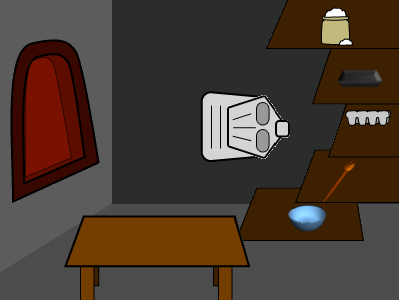
\includegraphics[width=\textwidth]{step0.png}
		\caption{Initial state}
		\label{img:initial}
	\end{subfigure}
	\centering
	\begin{subfigure}[b]{0.3\textwidth}
		\centering
		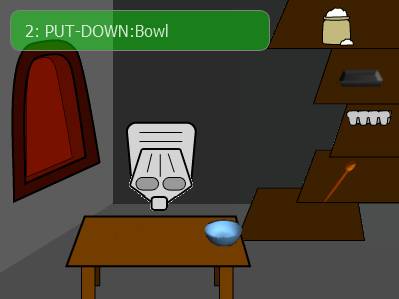
\includegraphics[width=\textwidth]{step1.png}
		\caption{Step 1}
		\label{img:bowl}
	\end{subfigure}
	\centering
	\begin{subfigure}[b]{0.3\textwidth}
		\centering
		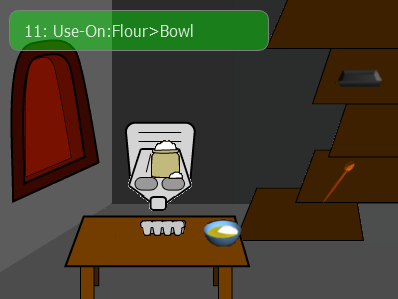
\includegraphics[width=\textwidth]{step3.png}
		\caption{Step 3}
		\label{img:ingredients}
	\end{subfigure}
	
	
	\centering
	\begin{subfigure}[b]{0.3\textwidth}
		\centering
		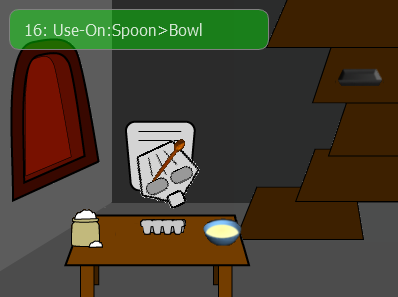
\includegraphics[width=\textwidth]{step4.png}
		\caption{Step 4}
		\label{img:batter}
	\end{subfigure}
	\centering
	\begin{subfigure}[b]{0.3\textwidth}
		\centering
		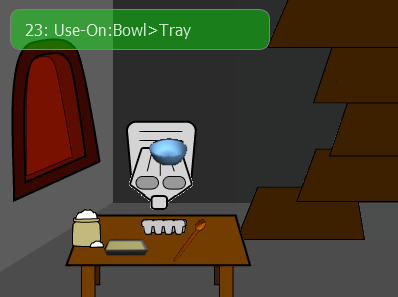
\includegraphics[width=\textwidth]{step5.png}
		\caption{Step 5}
		\label{img:tray}
	\end{subfigure}
	\centering
	\begin{subfigure}[b]{0.3\textwidth}
		\centering
		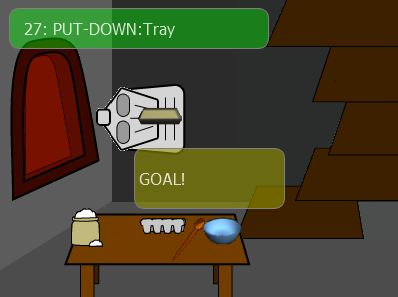
\includegraphics[width=\textwidth]{step6.png}
		\caption{Step 6}
		\label{img:goal}
	\end{subfigure}
	
	\caption{Presentation of different steps in the environment. \ref{img:initial} initial state, \ref{img:bowl} step 1: the bowl on the table, \ref{img:ingredients} step 3: both ingredients in the bowl, \ref{img:batter} step 4: ingredients mixed to obtain batter, \ref{img:tray} step 5: batter poured in the tray and \ref{img:goal} step 6 (success): tray with batter put in the oven. (Step 2: one ingredient in the bowl has been omitted for clarity)}
	\label{fig:states}
\end{figure}

\section{Results}

\section{Discussion}

\section{Summary}

